% !TeX spellcheck = en_US
\chapter{Appendix 1}%
%\Blindtext%
%
%

      \begin{sidewaysfigure}
      \centering
      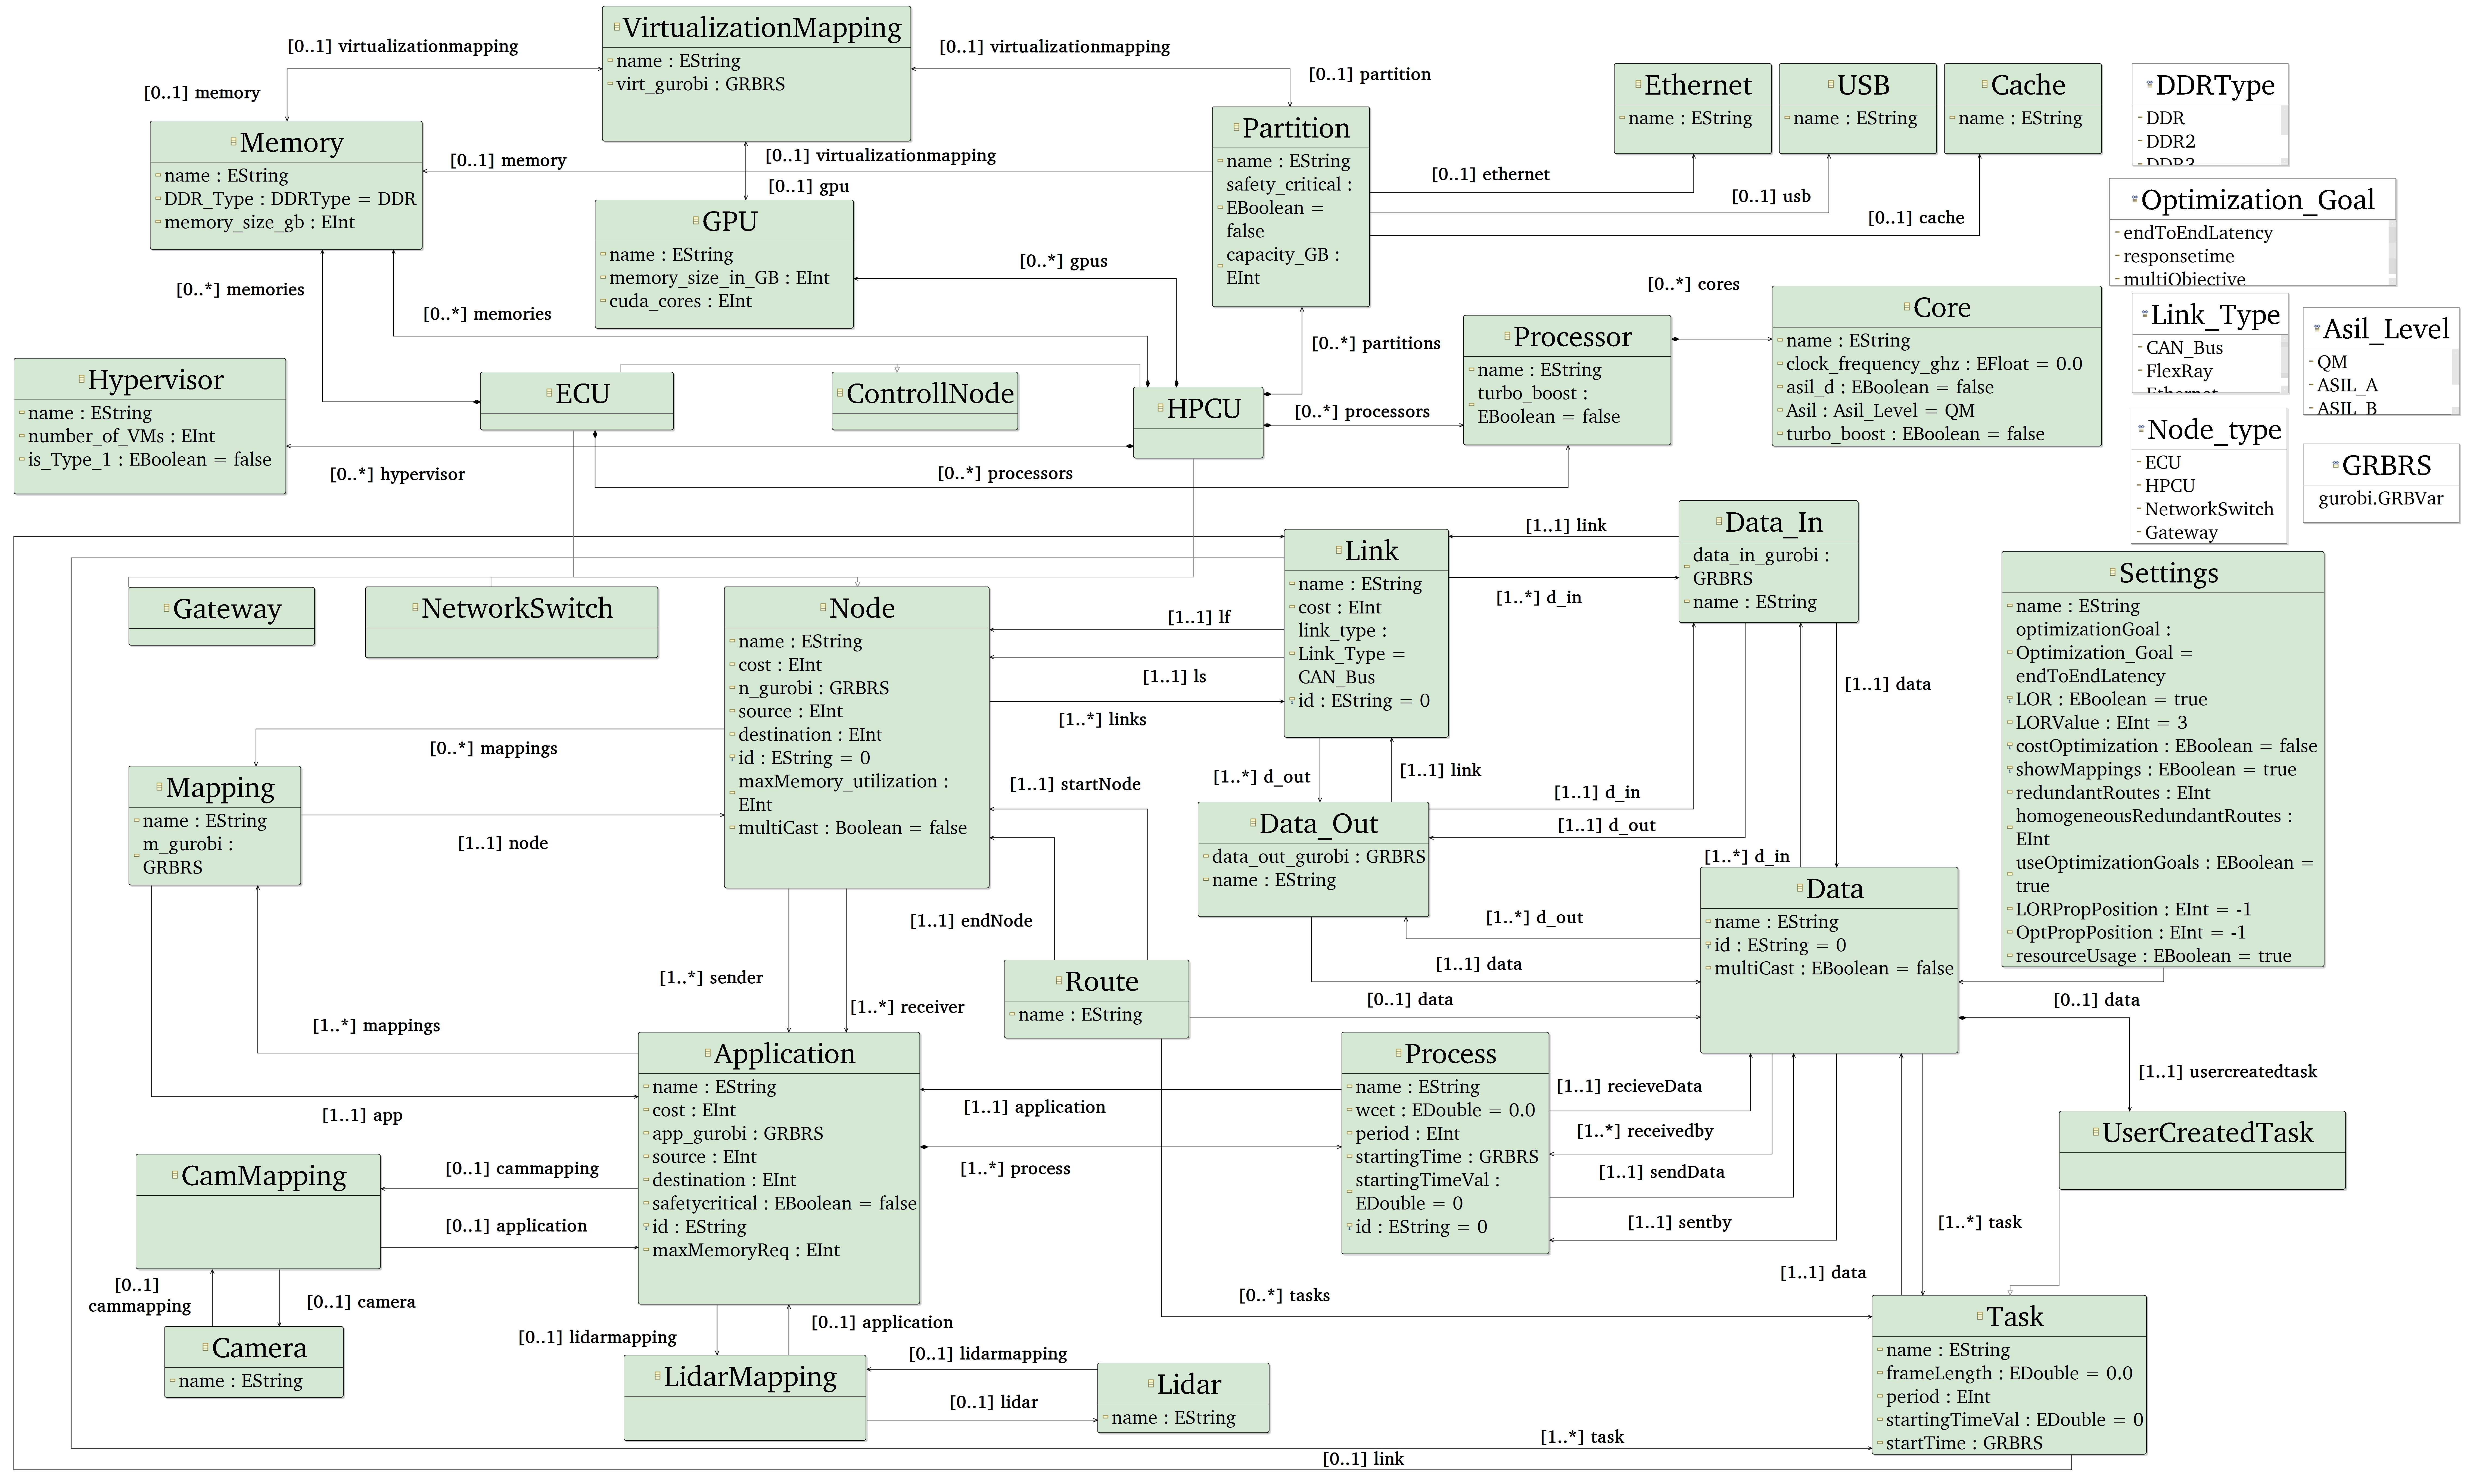
\includegraphics[angle = 360, width=1\textwidth]{figures/autoDesigner1_metamodel.jpg}
      %\captionsetup{angle=180}
      \caption{Object-oriented metamodel for the E/E Designer framework. The green boxes indicate the classes, and the white boxes represent the types of data and elements used within the classes.}
      \label{fig:metamodel}
      \end{sidewaysfigure}

    \begin{comment}
        
        \begin{table}
    	\begin{center}
    		\caption{Notation Reference.}
    		%\scriptsize
    		\begin{tabular}{@{}ccc@{}}
    			\toprule
    			&\textbf {MIP Input}\\
    			\midrule
    			%$H(A,D)$ & set of applications and communication messages\\[0.1cm]
    			%$n^{cz}$, $n^{nz}$  & control node and networking node\\
    			%$n^{cz_c}$ & single processor core of a control node\\
    			%$l_{a,b}$, 	$l_{b,a}$ &  directed link from $n_a$ to $n_b$ and directed link from $n_b$ to $n_a$\\
    			%$l_{b,a}$ &  directed link from $n_b$ to $n_a$ \\
    			$a^{asil}$ & ASIL level of an application \\[0.1cm]
    			$apn$ & a tolerable limit for number of assigned applications\\[0.1cm]
    			$bw$ & maximum amount of data transfer over a network link\\[0.1cm]
    			$c_i.p$, $c_i.fl$ & period and frame length of communication task $c_i$ \\[0.1cm]
    			$G(N,L)$ & set of vehicle topology nodes and full-duplex links \\[0.1cm]
    			$ipg$ & required time between network packets\\[0.1cm]
    			$pd$ & maximum processing delay of a communication frame\\[0.1cm]	
    			$rd$ & required time for preparation of receiving a packet by a $n^{cz}$ \\[0.1cm]					
    			$sd$ & required time for preparation of sending a packet by a $n^{cz}$ \\[0.1cm]
    			$sync$ & maximum difference between two any clocks in the system\\[0.1cm]
    			$t_i.p$, $t_i.e$& period and execution time of thread $t_i$, $i\in \mathbb{N}$ \\[0.1cm]
    			$t_{i{j}}^{s}$ & sender thread of application $a_j$ for communication message $d_i$, $j\in \mathbb{N}$ \\[0.1cm]
    			$t_{i{j}}^{r}$ & receiver thread of application $a_j$ for communication message $d_i$\\[0.1cm]
    			%$c_i.fl$ & frame length of communication task $c_i$ \\
    			\bottomrule
    			\toprule
    			&\textbf {MIP Decision Variables}\\
    			\midrule
    			$c_i.st$ & continuous: starting time of communication task $c_i$\\[0.1cm]
    			${d_i}^{in}$ & binary: 1 if communication message $d_i$ enters to a node via link\\[0.1cm]
    			${d_i}^{out}$ & binary: 1 if communication message $d_i$ goes out from a node via link\\[0.1cm]
    			${m_{ij}}$ & binary: 1 if application $a_j$ is executing on node $n_{i}^{cz}$\\[0.1cm]
    			${m_{ij}}^{s}$ & binary: 1 if sender thread $t$ from $a_j$ is executing on node $n_{i}^{cz}$\\[0.1cm]
    			${m_{ij}}^{r}$ & binary: 1 if receiver thread $t$ from $a_j$ is executing on node $n_{i}^{cz}$\\[0.1cm]
    			$t_i.st$ & continuous: starting time of thread $t_i$\\[0.1cm]
    			$v, r, q$ & binary: decided based on expression's solution \\[0.1cm]
    			\bottomrule
    			\toprule
    			&\textbf {Assistive Terms}\\
    			\midrule
    			$\mathcal{A}$ & a set of applications\\[0.1cm]
    			$A^{sc}$ & a set of safety-critical applications\\[0.1cm]
    			$a_i.t_{ij}$ & one/many threads $j$ belong to $a_i$\\[0.1cm]
    			$a_i.t_{ij}^{s}.d_i$ & sender thread $t_j$, which belongs to $a_i$, sending $d_i$ out\\[0.1cm]
    			$a_i.t_{ij}^{r}.d_i$ & receiver thread $t_j$, which belongs to $a_i$, receiving $d_i$\\[0.1cm]
    			$a_j.mu$ & memory usage of $a_j$ \\[0.1cm]
    			$\mathcal{C}$ & a set of communication tasks\\[0.1cm]
    			$c_i.st_{d_i}^{l_{j}}$ & starting time of $c_i$ related to $d_i$ over link $l_j$\\[0.1cm]
    			$\mathcal{D}$ & a set of communication messages\\[0.1cm]
    			$d_i.ch_i$ & message chain of $d_i$ containing sender and receiver threads for $d_i$\\[0.1cm]
    			$d_i.c_i$ & communication task of $d_i$\\[0.1cm]
    			$d_i.rt, d_i.el $ & response time and end-to-end latency of $d_i$ \\[0.1cm]		
    			$d_i^{out}.$$l_{a,b}^{n_a}$& message $d_i$ is sent out from $n_a$ over $l_{a,b}$\\[0.1cm]
    			$d_i^{in}.$$l_{b,a}^{n_a}$& message $d_i$ is received by $n_a$ over $l_{b,a}$\\[0.1cm]
    			$\mathcal{L}$ & a set of links\\[0.1cm]
    			$l_{a,b}$, $l_{b,a}$ &  directed link from $n_a$ to $n_b$ and directed link from $n_b$ to $n_a$\\[0.1cm]
    			$\mathcal{M}$ & a set of mapping variables\\[0.1cm]
    			${m_{ij}}.{a_j}^{n_{i}^{cz}}$ & mapping variable of $a_j$ running on $n_{i}^{cz}$ \\[0.1cm]
    			$m_{ij}^{s}.{a_j}^{n_i^{cz}}$ & mapping variable of sender thread from $a_j$ running on $n_{i}^{cz}$ \\[0.1cm]
    			$m_{ij}^{r}.{a_j}^{n_i^{cz}}$ & mapping variable of receiver thread from $a_j$ running on $n_{i}^{cz}$\\[0.1cm]
    			$\mathcal{N}$ & a set of nodes\\[0.1cm]
    			$n_{j}.d_p^{in}$& message $d_{p}$ enters to $n_{j}$ over a link\\[0.1cm]
    			$n_{j}.d_p^{out}$& message $d_{p}$ goes out from $n_{j}$ over a link\\[0.1cm]
    			$n^{cz}$, $n^{nz}$  & control node and networking node\\[0.1cm]
    			$n^{cz_c}$ & single processor core of a control node\\[0.1cm]
    			${n_i^{cz}}.m_{max}$ & maximum memory capacity of ${n_i^{cz}}$\\[0.1cm]
    			$nl$ & number of links related to each possible path \\[0.1cm]
    			$\mathcal{T}$ & a set of application threads\\[0.1cm]
    			$t_{i}^{s}.st_{d_i}$& starting time of sender $t_{i}$ sending $d_i$ \\[0.1cm]
    			$t_{i}^{r}.st_{d_i}$& starting time of receiver $t_{i}$ receiving $d_i$\\[0.1cm]
    			%${m_{ij}}.n_{i}^{cz}.a_j$ & mapping variable of receiver thread from $a_j$ running on $n_{i}^{cz}$ \\[0.1cm]
    			\bottomrule
    		\end{tabular}
    		\label{notations}
    	\end{center}
    \end{table}

    \end{comment}

    The following table illustrates the notation references for the variables used in the equations presented in Chapter \ref{method}.

                \begin{longtable}{@{}c c c c@{}}%{ p{.20\textwidth}  p{.40\textwidth} } 
                \caption{Notation Reference.}\\
                \label{notations}
                \endfirsthead
                \caption* {\textbf{Table \ref{notations}. Continued.}}\\\toprule
                \endhead
                \endfoot
                %\bottomrule
                \endlastfoot
 			\toprule
    			&\textbf {MIP Input}\\
    			\midrule
    			%$H(A,D)$ & set of applications and communication messages\\[0.1cm]
    			%$n^{cz}$, $n^{nz}$  & control node and networking node\\
    			%$n^{cz_c}$ & single processor core of a control node\\
    			%$l_{a,b}$, 	$l_{b,a}$ &  directed link from $n_a$ to $n_b$ and directed link from $n_b$ to $n_a$\\
    			%$l_{b,a}$ &  directed link from $n_b$ to $n_a$ \\
    			$a^{asil}$ & ASIL level of an application \\[0.1cm]
    			$apn$ & a tolerable limit for number of assigned applications\\[0.1cm]
    			$bw$ & maximum amount of data transfer over a network link\\[0.1cm]
    			$c_i.p$, $c_i.fl$ & period and frame length of communication task $c_i$ \\[0.1cm]
    			$G(N,L)$ & set of vehicle topology nodes and full-duplex links \\[0.1cm]
    			$ipg$ & required time between network packets\\[0.1cm]
    			$pd$ & maximum processing delay of a communication frame\\[0.1cm]	
    			$rd$ & required time for preparation of receiving a packet by a $n^{cz}$ \\[0.1cm]					
    			$sd$ & required time for preparation of sending a packet by a $n^{cz}$ \\[0.1cm]
    			$sync$ & maximum difference between two any clocks in the system\\[0.1cm]
    			$t_i.p$, $t_i.e$& period and execution time of thread $t_i$, $i\in \mathbb{N}$ \\[0.1cm]
    			$t_{i{j}}^{s}$ & sender thread of application $a_j$ for communication message $d_i$, $j\in \mathbb{N}$ \\[0.1cm]
    			$t_{i{j}}^{r}$ & receiver thread of application $a_j$ for communication message $d_i$\\[0.1cm]
    			%$c_i.fl$ & frame length of communication task $c_i$ \\
    			\bottomrule
    			\toprule
    			&\textbf {MIP Decision Variables}\\
    			\midrule
    			$c_i.st$ & continuous: starting time of communication task $c_i$\\[0.1cm]
    			${d_i}^{in}$ & binary: 1 if communication message $d_i$ enters to a node via link\\[0.1cm]
    			${d_i}^{out}$ & binary: 1 if communication message $d_i$ goes out from a node via link\\[0.1cm]
    			${m_{ij}}$ & binary: 1 if application $a_j$ is executing on node $n_{i}^{cz}$\\[0.1cm]
    			${m_{ij}}^{s}$ & binary: 1 if sender thread $t$ from $a_j$ is executing on node $n_{i}^{cz}$\\[0.1cm]
    			${m_{ij}}^{r}$ & binary: 1 if receiver thread $t$ from $a_j$ is executing on node $n_{i}^{cz}$\\[0.1cm]
    			$t_i.st$ & continuous: starting time of thread $t_i$\\[0.1cm]
    			$v, r, q$ & binary: decided based on expression's solution \\[0.1cm]
    			\bottomrule
    			\toprule
    			&\textbf {Assistive Terms}\\
    			\midrule
    			$\mathcal{A}$ & a set of applications\\[0.1cm]
    			$A^{sc}$ & a set of safety-critical applications\\[0.1cm]
    			$a_i.t_{ij}$ & one/many threads $j$ belong to $a_i$\\[0.1cm]
    			$a_i.t_{ij}^{s}.d_i$ & sender thread $t_j$, which belongs to $a_i$, sending $d_i$ out\\[0.1cm]
    			$a_i.t_{ij}^{r}.d_i$ & receiver thread $t_j$, which belongs to $a_i$, receiving $d_i$\\[0.1cm]
    			$a_j.mu$ & memory usage of $a_j$ \\[0.1cm]
    			$\mathcal{C}$ & a set of communication tasks\\[0.1cm]
    			$c_i.st_{d_i}^{l_{j}}$ & starting time of $c_i$ related to $d_i$ over link $l_j$\\[0.1cm]
    			$\mathcal{D}$ & a set of communication messages\\[0.1cm]
    			$d_i.ch_i$ & message chain of $d_i$ containing sender and receiver threads for $d_i$\\[0.1cm]
    			$d_i.c_i$ & communication task of $d_i$\\[0.1cm]
    			$d_i.rt, d_i.el $ & response time and end-to-end latency of $d_i$ \\[0.1cm]		
    			$d_i^{out}.$$l_{a,b}^{n_a}$& message $d_i$ is sent out from $n_a$ over $l_{a,b}$\\[0.1cm]
    			$d_i^{in}.$$l_{b,a}^{n_a}$& message $d_i$ is received by $n_a$ over $l_{b,a}$\\[0.1cm]
    			$\mathcal{L}$ & a set of links\\[0.1cm]
    			$l_{a,b}$, $l_{b,a}$ &  directed link from $n_a$ to $n_b$ and directed link from $n_b$ to $n_a$\\[0.1cm]
    			$\mathcal{M}$ & a set of mapping variables\\[0.1cm]
    			${m_{ij}}.{a_j}^{n_{i}^{cz}}$ & mapping variable of $a_j$ running on $n_{i}^{cz}$ \\[0.1cm]
    			$m_{ij}^{s}.{a_j}^{n_i^{cz}}$ & mapping variable of sender thread from $a_j$ running on $n_{i}^{cz}$ \\[0.1cm]
    			$m_{ij}^{r}.{a_j}^{n_i^{cz}}$ & mapping variable of receiver thread from $a_j$ running on $n_{i}^{cz}$\\[0.1cm]
    			$\mathcal{N}$ & a set of nodes\\[0.1cm]
    			$n_{j}.d_p^{in}$& message $d_{p}$ enters to $n_{j}$ over a link\\[0.1cm]
    			$n_{j}.d_p^{out}$& message $d_{p}$ goes out from $n_{j}$ over a link\\[0.1cm]
    			$n^{cz}$, $n^{nz}$  & control node and networking node\\[0.1cm]
    			$n^{cz_c}$ & single processor core of a control node\\[0.1cm]
    			${n_i^{cz}}.m_{max}$ & maximum memory capacity of ${n_i^{cz}}$\\[0.1cm]
    			$nl$ & number of links related to each possible path \\[0.1cm]
    			$\mathcal{T}$ & a set of application threads\\[0.1cm]
    			$t_{i}^{s}.st_{d_i}$& starting time of sender $t_{i}$ sending $d_i$ \\[0.1cm]
    			$t_{i}^{r}.st_{d_i}$& starting time of receiver $t_{i}$ receiving $d_i$\\[0.1cm]
    			%${m_{ij}}.n_{i}^{cz}.a_j$ & mapping variable of receiver thread from $a_j$ running on $n_{i}^{cz}$ \\[0.1cm]
    			\bottomrule
%\caption{Your caption here} % needs to go inside longtable environment
%\label{tab:myfirstlongtable}
\end{longtable}

    In the following, a visual representation of the object-oriented metamodel created for the computer-assisted tool introduced in this thesis is provided. 